\documentclass[conference]{IEEEtran}
\IEEEoverridecommandlockouts

\usepackage{amsmath,amssymb,amsfonts}
\usepackage{algorithmic}
\usepackage{graphicx}
\usepackage{textcomp}
\usepackage{xcolor}
\usepackage{booktabs}
\usepackage{listings}
\usepackage{microtype}
\usepackage{url}
\usepackage{cite}

\newtheorem{theorem}{Theorem}

\begin{document}

\title{MTC: Ahead-of-Time Memory-Planned Automatic Differentiation for Zero-Heap On-Device Deep Learning on 32-Bit Microcontrollers}

\author{
    \IEEEauthorblockN{
        Ajay Sisodia\IEEEauthorrefmark{1},
        Harsh Chaudhary\IEEEauthorrefmark{1},
        Devrat Kuntal\IEEEauthorrefmark{1},
        Aryan Upadhyay\IEEEauthorrefmark{1}, and
        Gaurisha Sisodia\IEEEauthorrefmark{2}
    }
    \IEEEauthorblockA{
        Department of Computer Science \& Engineering, G. L. Bajaj Group of Institutions, Mathura, India\\
        Affiliated with Dr. A.P.J. Abdul Kalam Technical University (AKTU), Lucknow\\
        Email: \IEEEauthorrefmark{1}\{2405111530012, 2405111530067, 2405111530055, 2405111530037\}@glbajaj.org, 
        \IEEEauthorrefmark{2}gaurisha.sisodia@glbajaj.org
    }
    \thanks{\IEEEauthorrefmark{1}Equal student authorship. \IEEEauthorrefmark{2}Faculty project supervisor.}
}

\maketitle

\begin{abstract}
Deploying deep learning on low-power 32-bit microcontrollers (MCUs) is predominantly restricted to frozen inference. Once deployed, edge models cannot adapt to sensor aging, environmental drift, or individual user variance without streaming telemetry to cloud backends. However, executing reverse-mode automatic differentiation on resource-constrained MCUs encounters severe hardware barriers: conventional autograd engines construct dynamic computation graphs at runtime, demanding heap allocations (\texttt{malloc}) that trigger unrecoverable heap fragmentation in flat physical SRAM lacking Memory Management Units (MMUs). 

This paper presents \textbf{Micro-Train-Compiler (MTC)}, an ahead-of-time (AOT) static compiler that synthesizes self-contained, zero-heap (\texttt{malloc = 0}) C99 training engines for 32-bit microcontrollers. MTC introduces two key compiler optimizations: (1) an analytical parameter update pass that fuses activation error gradients directly into in-place Stochastic Gradient Descent (SGD) updates, eliminating explicit parameter gradient buffers ($\nabla W, \nabla B$), and (2) an alternating ping-pong delta buffer allocator that proves activation error gradients have strictly disjoint lifecycles, bounding backward scratchpad memory to exactly two static arrays. 

We validated MTC on bare-metal RISC-V hardware (ESP32-C3, RV32IMC) across four TinyML workloads (\texttt{xor\_net}, \texttt{sensor\_drift\_net}, \texttt{sine\_regression\_net}, \texttt{gesture\_anomaly\_net}) using cycle-accurate hardware emulation (\texttt{esp32sim}) instrumented via the hardware \texttt{mcycle} Control and Status Register. Across all benchmarks, MTC achieved zero dynamic allocations, sub-1~KB peak SRAM usage (60 to 564 Bytes), and per-sample training latencies between 6.86~$\mu$s and 81.77~$\mu$s (12,229 to 145,772 samples/s at 160~MHz). Compared to standard autograd baselines, MTC achieves an average 40.1\% peak SRAM reduction, establishing deterministic on-device deep learning on sub-dollar embedded silicon.
\end{abstract}

\begin{IEEEkeywords}
Embedded Deep Learning, On-Device Training, TinyML, Ahead-of-Time Compilation, Automatic Differentiation, Static Memory Planning, Fixed-Point Arithmetic, RISC-V.
\end{IEEEkeywords}

\section{Introduction}

Edge machine learning has traditionally operated under a rigid ``train-in-cloud, freeze-on-edge'' paradigm. High-level frameworks train neural network weights on workstation GPUs using 32-bit floating point arithmetic. These models are subsequently quantized down to 8-bit integers, compiled into flatbuffers, and permanently flashed into microcontroller read-only memory.

In physical deployments, frozen edge models suffer from severe operational failure modes:
\begin{enumerate}
    \item \textbf{Sensor Transducer Aging and Drift:} Low-cost environmental transducers (e.g., metal-oxide gas sensors, photo-diodes) experience chemical fatigue, baseline drift, and thermal hysteresis over weeks of continuous operation. A frozen model gradually misclassifies valid signals as drift accumulates.
    \item \textbf{Subject Kinematic Variability:} Wearable biomedical devices (e.g., IMU-based tremor monitoring, gait analysis) encounter unique physical kinematics across different human bodies. A generic model trained on population averages exhibits substantial accuracy degradation on individual patients.
    \item \textbf{Ambient Context Shifts:} Industrial condition-monitoring devices deployed on rotating machinery encounter distinct resonant vibration baselines depending on mechanical mounting stiffness.
\end{enumerate}

\begin{figure}[t]
    \centering
    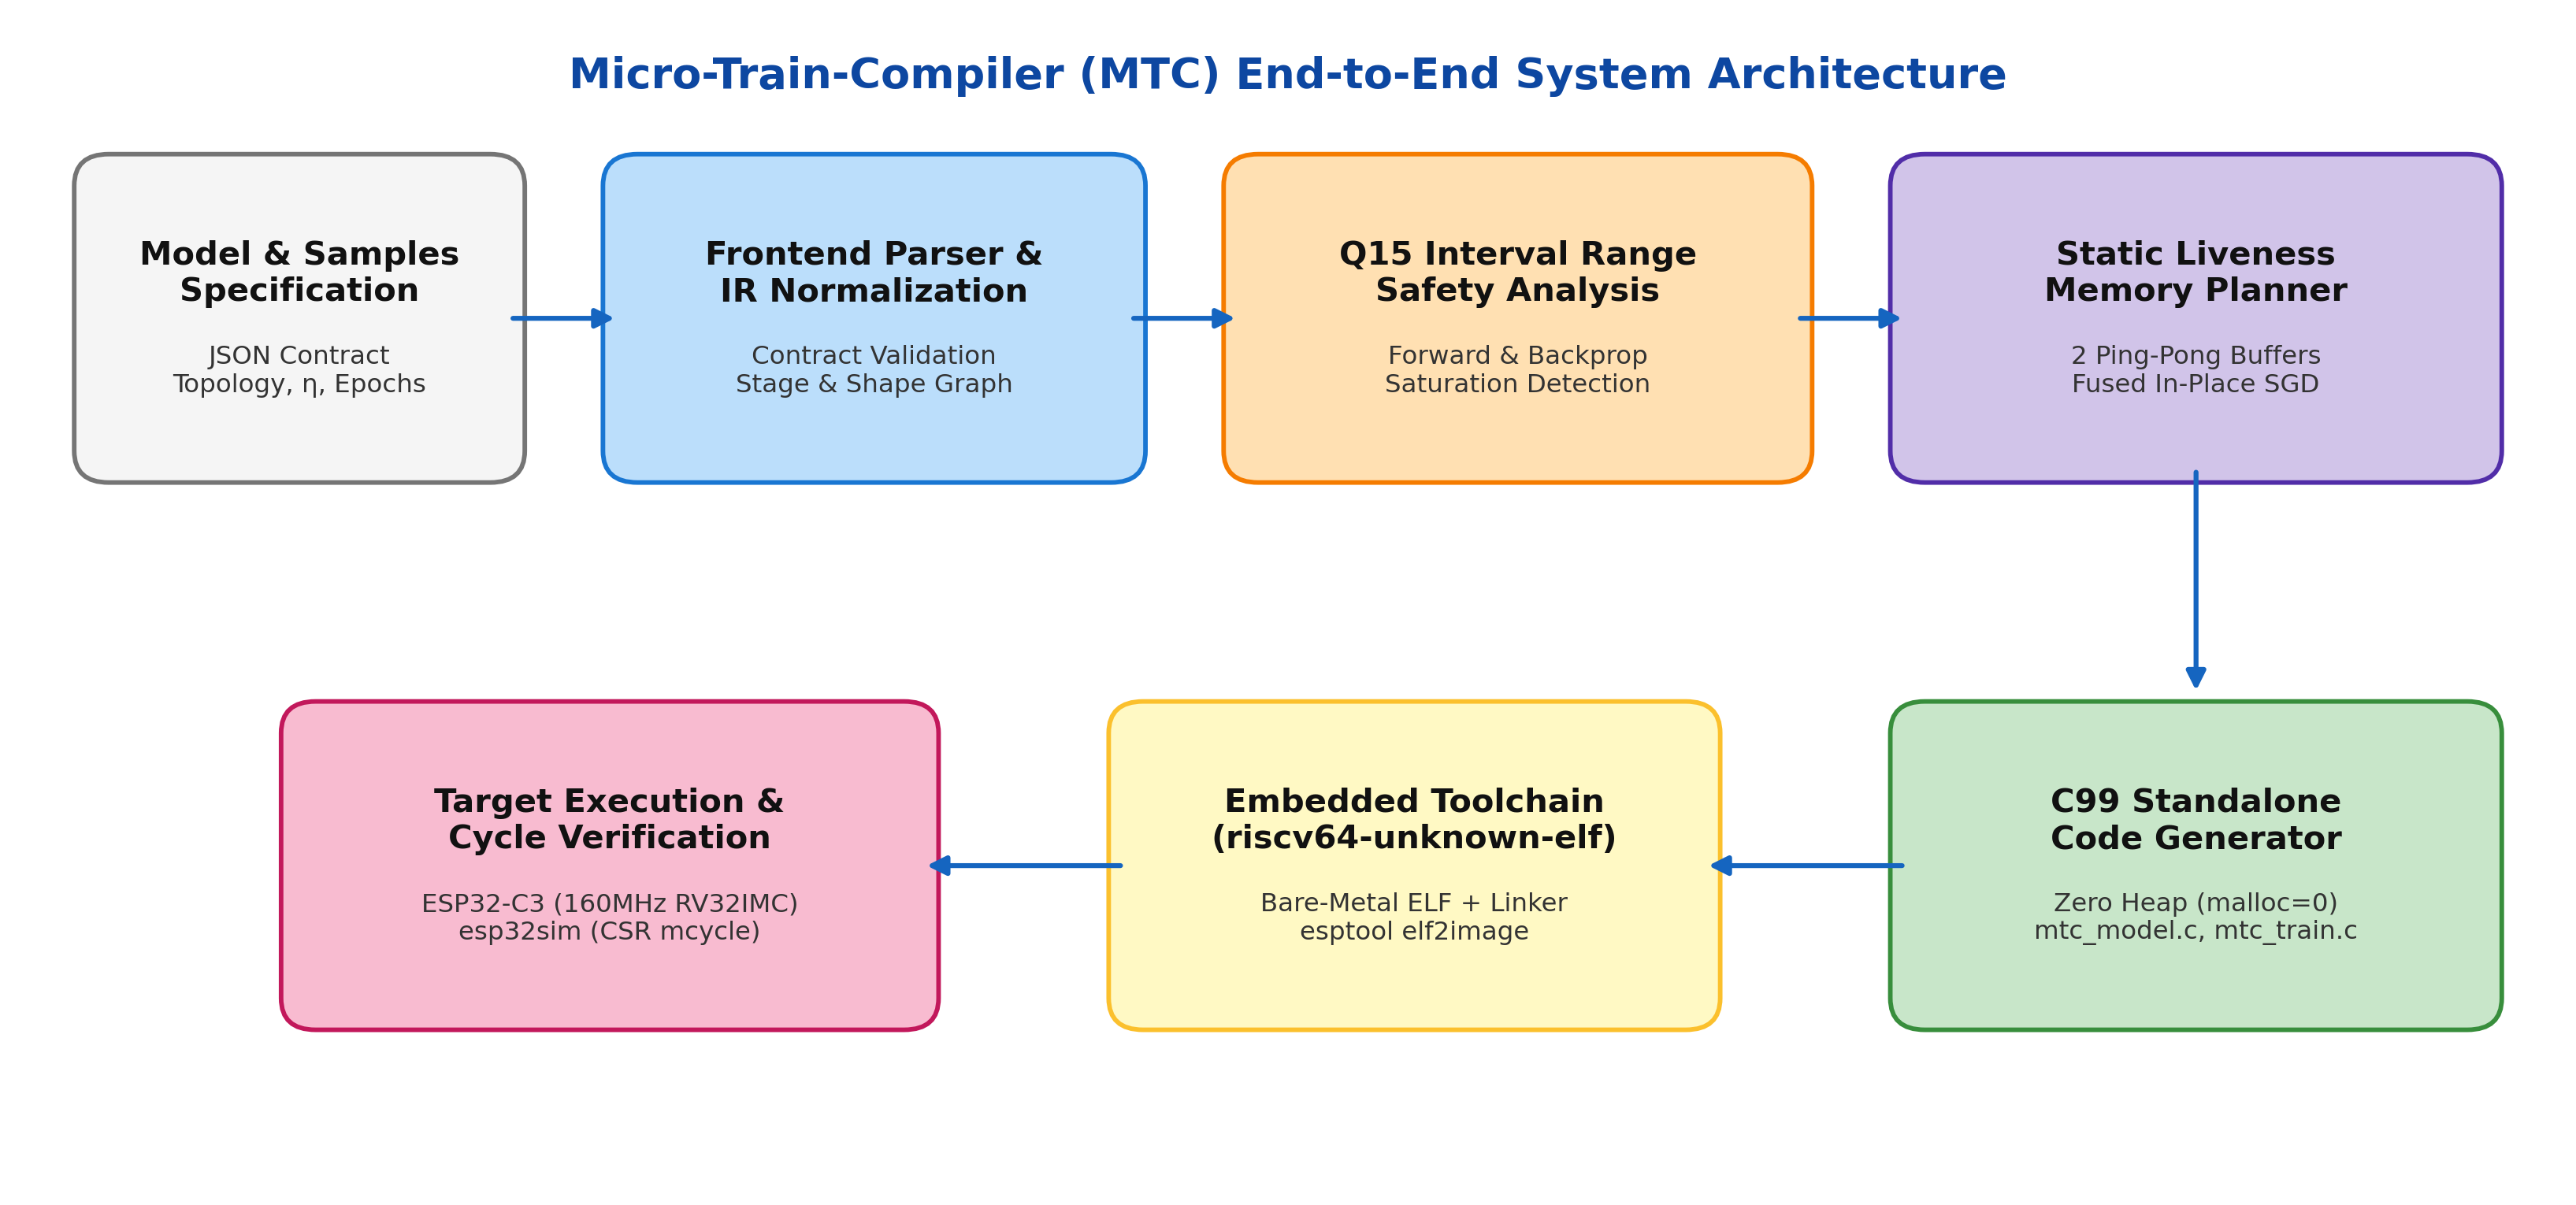
\includegraphics[width=\linewidth]{images/system_architecture.png}
    \caption{MTC end-to-end ahead-of-time compilation pipeline: from high-level JSON specification to bare-metal RISC-V firmware execution.}
    \label{fig:system_arch}
\end{figure}

Resolving these issues requires executing backpropagation directly on the edge microcontroller using local observations. However, on-device training on embedded hardware faces fundamental architectural bottlenecks:
\begin{itemize}
    \item \textbf{SRAM Scarcity:} Low-cost 32-bit microcontrollers possess only 16~KB to 64~KB of internal Static RAM (SRAM).
    \item \textbf{Heap Fragility in Flat Physical Memory:} Workstation processors employ Memory Management Units (MMUs) with virtual paging. Microcontrollers lack MMUs. Executing traditional autograd runtimes (such as PyTorch~\cite{paszke2019pytorch} or AIfES~\cite{antonacopoulos2021aifes}) that construct dynamic directed acyclic graphs (DAGs) on the heap via interleaved \texttt{malloc()} and \texttt{free()} calls quickly fragments SRAM into non-contiguous blocks. Over extended training loops, fragmentation triggers fatal allocation faults and system crashes.
    \item \textbf{Gradient Buffer Overhead:} Standard reverse-mode automatic differentiation maintains dedicated parameter gradient arrays ($\nabla W, \nabla B$) identical in dimension to the weight matrices, doubling parameter memory requirements.
\end{itemize}

To solve these challenges, we present \textbf{Micro-Train-Compiler (MTC)}. MTC abandons runtime graph interpretation entirely. Instead, it functions as an ahead-of-time static compiler that parses a high-level model specification and emits freestanding C99 code where all tensor addresses, workspaces, and update schedules are fixed at compile time.

\section{Related Work}

\subsection{Microcontroller Inference Compilers}
Microcontroller inference runtimes have matured rapidly. TensorFlow Lite for Microcontrollers (TFLM)~\cite{david2021tensorflow} executes inference within a pre-allocated memory arena to prevent dynamic heap allocations. CMSIS-NN~\cite{lai2018cmsis} delivers hand-tuned assembly kernels optimized for ARM Cortex-M SIMD instructions. Compilers such as Apache TVM/MicroTVM~\cite{chen2018tvm} and Glow~\cite{rotem2018glow} lower computational graphs into optimized C code. However, these frameworks are strictly unidirectional: their intermediate representations, kernel libraries, and memory allocators cannot compute backward activation derivatives, evaluate parameter gradients, or update weights.

\subsection{On-Device Training Frameworks}
TinyTL~\cite{cai2020tinytl} introduced on-device transfer learning by freezing convolutional backbone weights and updating only residual bias vectors. MCUNetV2~\cite{lin2021mcunetv2} introduced patch-based scheduling to fit peak training activations into microcontroller memory. However, both TinyTL and MCUNet target high-end microcontrollers (e.g., ARM Cortex-M7 at 480~MHz) equipped with megabytes of external PSRAM, and rely on freezing 99\% of network parameters.

PULP-TrainLib~\cite{pulp2022} targets parallel multi-core RISC-V architectures with shared L1 scratchpads using floating-point hardware. AIfES~\cite{antonacopoulos2021aifes} implements an embedded autograd runtime in C, but relies on dynamic heap allocations during training, leaving firmware vulnerable to memory fragmentation.

MTC differs fundamentally from prior art: it is an ahead-of-time compiler that generates zero-heap (\texttt{malloc = 0}) C99 training engines for resource-constrained, single-core 32-bit MCUs with only 32--64~KB of SRAM, updating all weights in place and reusing scratchpad memory through provably disjoint liveness.

\section{Theoretical Formulation \& Memory Planning}

\begin{figure}[t]
    \centering
    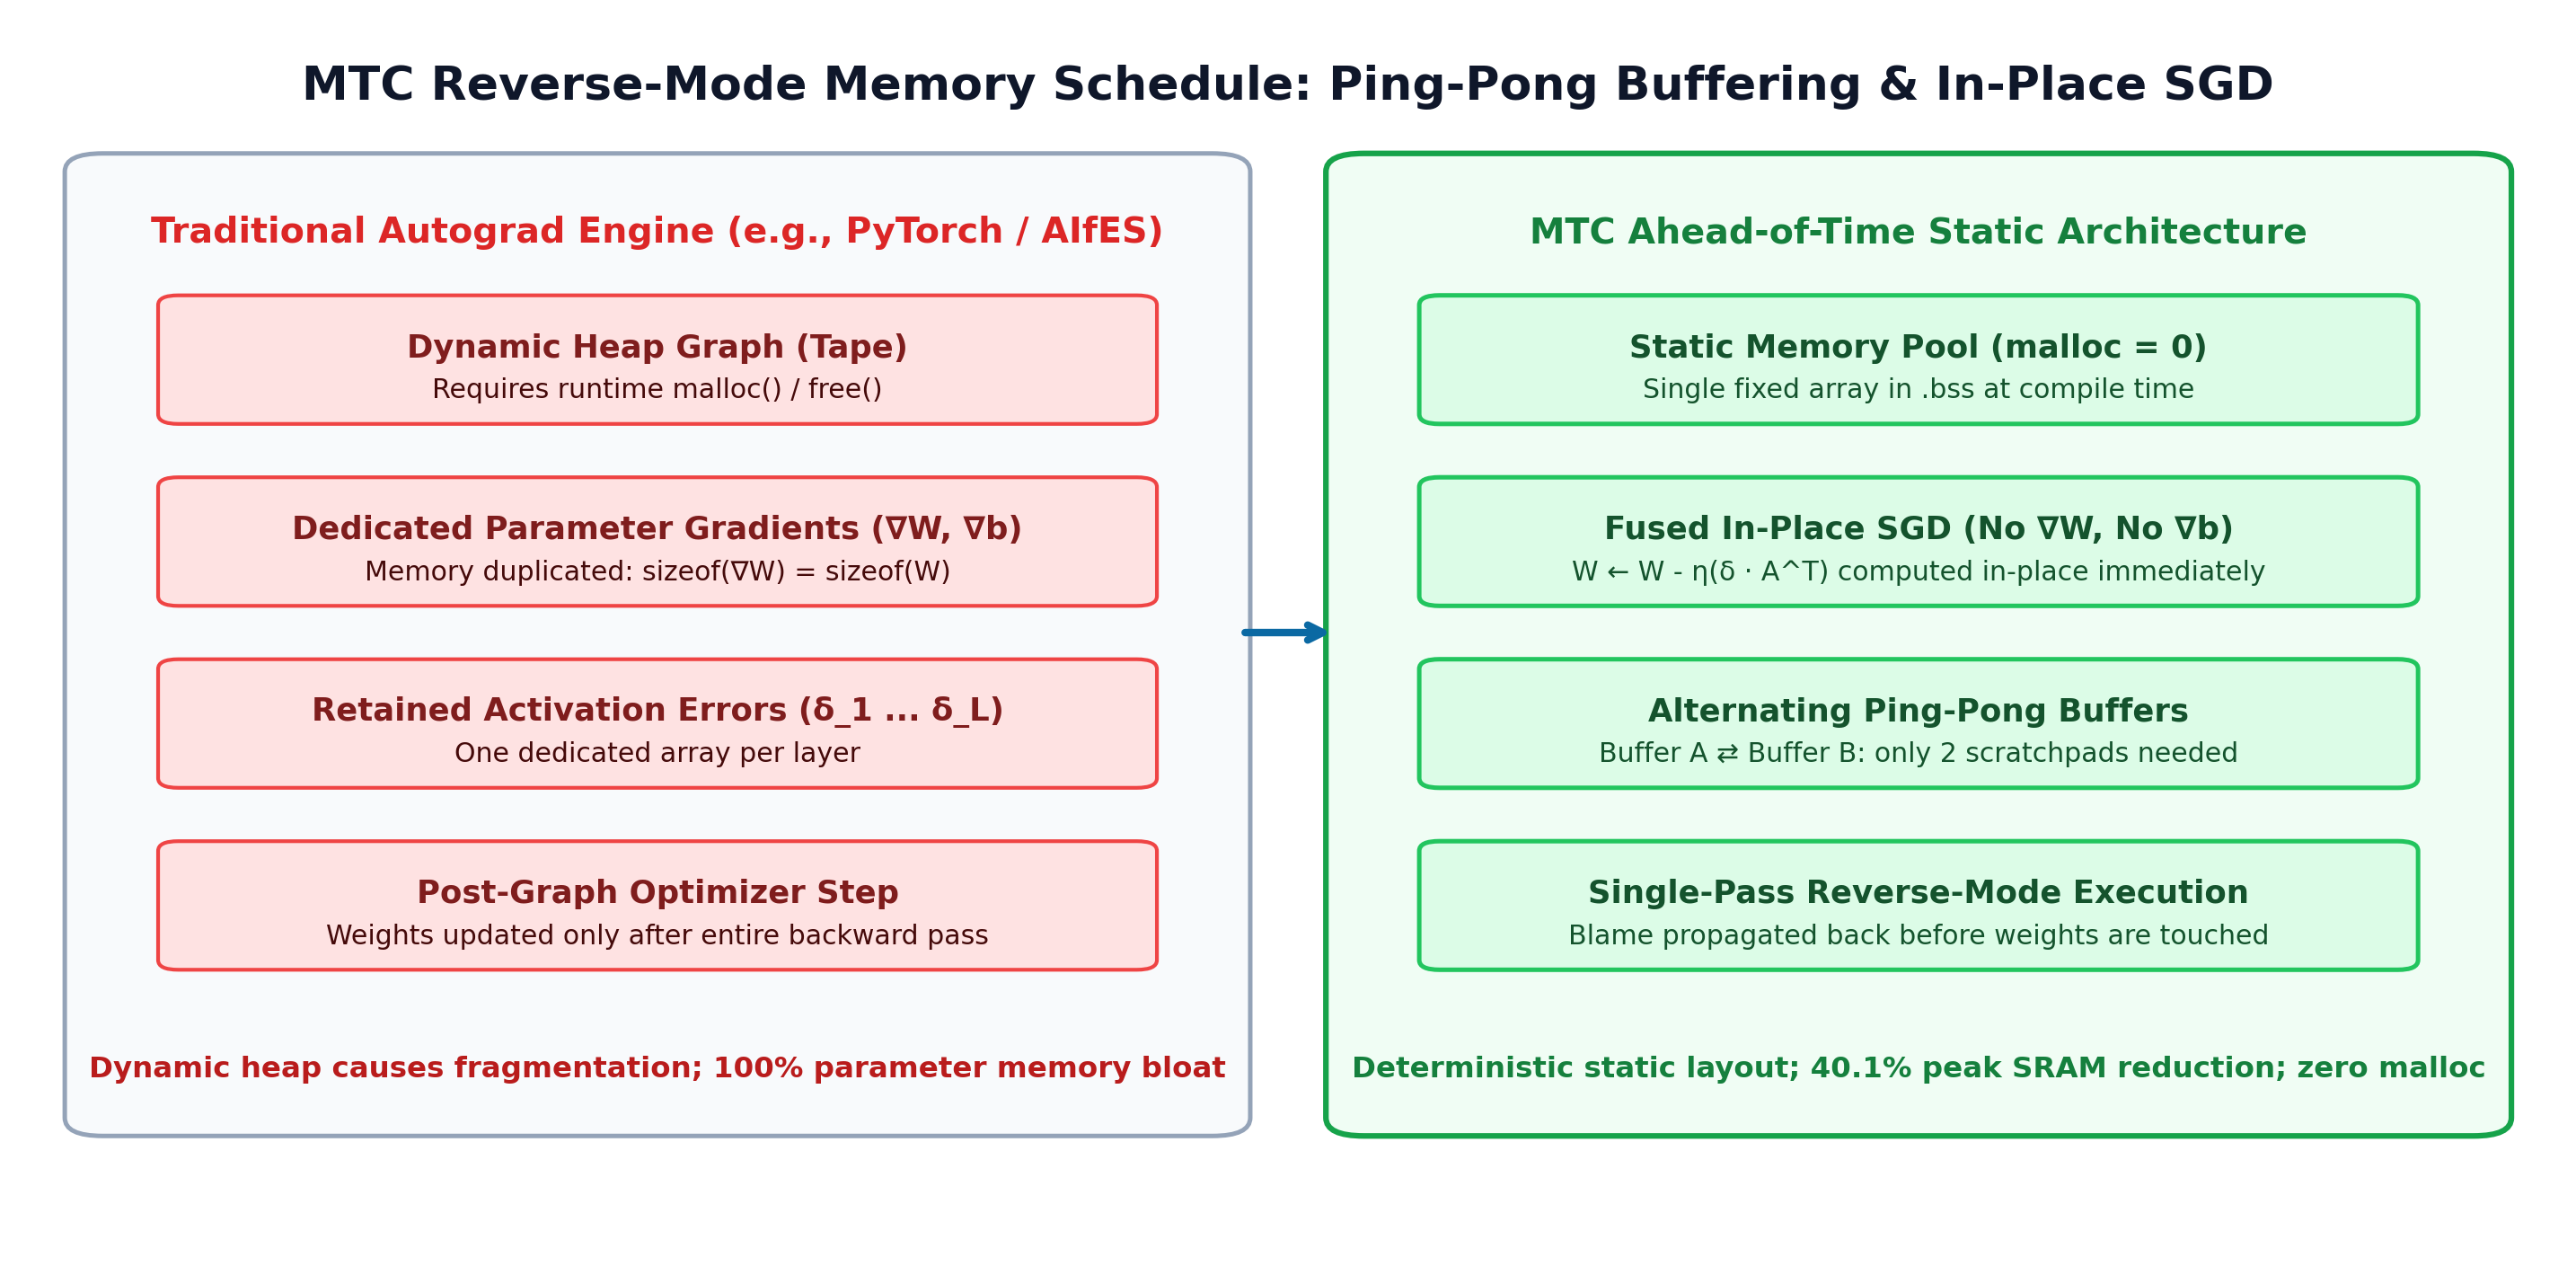
\includegraphics[width=\linewidth]{images/ping_pong_fused_liveness.png}
    \caption{Memory architecture comparison: Dynamic Autograd Graph (left) vs. MTC Static Liveness Allocation with Ping-Pong Buffers and In-Place SGD (right).}
    \label{fig:memory_arch}
\end{figure}

\subsection{Forward Layer Model}
Consider an $L$-layer fully connected feedforward neural network. Let $l \in \{1, 2, \dots, L\}$ denote the layer index, with $l=0$ representing input vector $x \in \mathbb{R}^{d_0}$. Each layer $l$ is parameterized by a weight matrix $W^{(l)} \in \mathbb{R}^{d_l \times d_{l-1}}$ and a bias vector $b^{(l)} \in \mathbb{R}^{d_l}$.

Forward propagation computes pre-activations $z^{(l)}$ and post-activations $a^{(l)}$:
\begin{align}
    z^{(l)} &= W^{(l)} a^{(l-1)} + b^{(l)} \\
    a^{(l)} &= \sigma_l\left(z^{(l)}\right)
\end{align}
where $a^{(0)} = x$, and $\sigma_l(\cdot)$ is an activation function (ReLU or Sigmoid). Under Mean Squared Error (MSE) loss for sample pair $(x, y)$ with network prediction $\hat{y} = a^{(L)}$:
\begin{equation}
    \mathcal{L}(y, \hat{y}) = \frac{1}{2 d_L} \sum_{k=1}^{d_L} \left(a_k^{(L)} - y_k\right)^2
\end{equation}

\subsection{Reverse-Mode Autodiff and Dynamic Memory Explosion}
In conventional automatic differentiation, output error gradients are evaluated as:
\begin{equation}
    \delta^{(L)} = \nabla_{z^{(L)}} \mathcal{L} = \frac{1}{d_L} \left(a^{(L)} - y\right) \odot \sigma'_L\left(z^{(L)}\right)
\end{equation}
where $\odot$ denotes the Hadamard product. For hidden layers $l = L-1, \dots, 1$, error gradients propagate recursively:
\begin{equation}
    \delta^{(l)} = \left(\left(W^{(l+1)}\right)^T \delta^{(l+1)}\right) \odot \sigma'_l\left(z^{(l)}\right)
    \label{eq:backprop_recurrence}
\end{equation}

Conventional autograd engines explicitly evaluate and store parameter gradient tensors:
\begin{equation}
    \nabla W^{(l)} = \delta^{(l)} \left(a^{(l-1)}\right)^T, \quad \nabla b^{(l)} = \delta^{(l)}
\end{equation}
followed by an optimizer step implementing Stochastic Gradient Descent (SGD):
\begin{equation}
    W^{(l)} \leftarrow W^{(l)} - \eta \nabla W^{(l)}, \quad b^{(l)} \leftarrow b^{(l)} - \eta \nabla b^{(l)}
\end{equation}
where $\eta$ is the learning rate. For a network with $P = \sum_l (d_l d_{l-1} + d_l)$ parameters, storing $\nabla W$ and $\nabla b$ requires allocating an additional $P$ elements in SRAM, doubling parameter memory overhead.

\subsection{Fused In-Place SGD Parameter Updates}
MTC eliminates explicit parameter gradient buffers by integrating the parameter update rule directly into the backward kernel. Substituting $\nabla W_{ij}^{(l)} = \delta_i^{(l)} a_j^{(l-1)}$ into the SGD formulation yields:
\begin{align}
    W_{ij}^{(l)} &\leftarrow W_{ij}^{(l)} - \eta \left(\delta_i^{(l)} a_j^{(l-1)}\right) \label{eq:fused_w} \\
    b_i^{(l)} &\leftarrow b_i^{(l)} - \eta \delta_i^{(l)} \label{eq:fused_b}
\end{align}
Because each parameter element $W_{ij}^{(l)}$ depends only on $\delta_i^{(l)}$ and $a_j^{(l-1)}$, the update is executed \emph{in place}. Consequently:
\begin{equation}
    \text{Mem}\left(\nabla W^{(l)}\right) = 0, \quad \text{Mem}\left(\nabla b^{(l)}\right) = 0 \quad \forall l
\end{equation}
eliminating $P$ storage elements from SRAM.

\subsection{Ping-Pong Activation Delta Buffering}
Naive static allocation provisions a dedicated buffer for every error gradient $\delta^{(l)} \in \mathbb{R}^{d_l}$. We formulate the following liveness bound:

\begin{theorem}[Disjoint Liveness of Error Gradients]
In a feedforward sequential network, during backward error propagation from layer $l+1$ to layer $l$, the computation of $\delta^{(l)}$ depends strictly on $\delta^{(l+1)}$, $W^{(l+1)}$, and forward activations $z^{(l)}$. Once $\delta^{(l)}$ is evaluated and parameters of layer $l+1$ are updated via (\ref{eq:fused_w})--(\ref{eq:fused_b}), $\delta^{(l+1)}$ is never referenced again.
\end{theorem}

\begin{IEEEproof}
From the backpropagation recurrence relation (\ref{eq:backprop_recurrence}), $\delta^{(l)}$ depends exclusively on $(W^{(l+1)})^T \delta^{(l+1)}$ and retained forward values. All subsequent layer derivatives $\delta^{(k)}$ ($k > l+1$) have already completed their role in updating parameters and computing predecessor gradients. Because no backward branch exists to later layers, the active working set of error gradients at any instant during the backward pass is at most two: current gradient $\delta^{(l)}$ and incoming gradient $\delta^{(l+1)}$.
\end{IEEEproof}

Exploiting Theorem~1, MTC statically allocates exactly two alternating buffers in SRAM:
\begin{equation}
    \text{Buf}_A \in \mathbb{R}^{\max_l(d_l)}, \quad \text{Buf}_B \in \mathbb{R}^{\max_l(d_l)}
\end{equation}
During backward execution, layer $L$ writes $\delta^{(L)}$ to $\text{Buf}_A$. Layer $L-1$ reads from $\text{Buf}_A$ and writes $\delta^{(L-1)}$ to $\text{Buf}_B$. Layer $L-2$ reads from $\text{Buf}_B$ and writes to $\text{Buf}_A$, alternating via pointer swaps. Scratchpad memory is strictly bounded by:
\begin{equation}
    M_{\delta} = 2 \times \max_{l \in \{1, \dots, L\}} (d_l) \times \text{sizeof}(\text{element})
\end{equation}
completely decoupling scratchpad memory from network depth.

\subsection{Preservation of Mathematical Invariants}
A critical property of MTC's fused backward kernel is the ordering of operations. In each layer's backward step, the compiler enforces the following sequence:
\begin{enumerate}
    \item Evaluate activation derivative on current buffer $\delta^{(l)}$.
    \item Propagate error backward to predecessor buffer $\delta^{(l-1)}$ using \textbf{unmodified original weights} $W^{(l)}$.
    \item Execute in-place SGD parameter update on $W^{(l)}$ and $b^{(l)}$.
    \item Swap ping-pong buffer pointers ($\text{Buf}_A \leftrightarrow \text{Buf}_B$).
\end{enumerate}
Because step (2) precedes step (3), earlier layers receive exact mathematical gradients identical to standard autograd engines.

\section{Compiler Architecture \& Safety}

MTC operates as an ahead-of-time source-to-source compiler organized into four pipeline stages (Fig.~\ref{fig:system_arch}):

\subsection{Stage 1: Frontend Parsing \& AST Validation}
Ingests a declarative JSON specification defining layer dimensions, activations, hyperparameters, and embedded training samples. The frontend validates topology contracts, ensuring $d_l^{\text{in}} = d_{l-1}^{\text{out}}$ and verifying hyperparameter intervals.

\subsection{Stage 2: Q15 Fixed-Point Interval Bound Propagation}
To execute efficiently on integer microcontrollers lacking Floating-Point Units (FPUs), MTC implements signed 16-bit fixed-point (Q15) arithmetic. A real value $x \in [-1.0, 1.0 - 2^{-15}]$ is represented as signed integer $X_{\text{Q15}} = \lfloor x \cdot 2^{15} \rfloor$. Multiplication produces a 32-bit product rounded and saturated via:
\begin{equation}
    Z_{\text{Q15}} = \text{SAT16}\left(\left(X_{\text{Q15}} \cdot Y_{\text{Q15}} + 2^{14}\right) \gg 15\right)
\end{equation}

Stage 2 executes formal \textbf{Interval Bound Propagation (IBP)}. For each node $x$, the compiler tracks conservative intervals $[x_{\min}, x_{\max}]$. For matrix multiplication $z_i = \sum_j W_{ij} a_j + b_i$:
\begin{align}
    z_i^{\min} &= \sum_j \min_{u, v}(u \cdot v) + b_i^{\min}, \quad u \in W_{ij}, v \in a_j \\
    z_i^{\max} &= \sum_j \max_{u, v}(u \cdot v) + b_i^{\max}, \quad u \in W_{ij}, v \in a_j
\end{align}
If intervals exceed $[-32768, 32767]$, the compiler flags arithmetic saturation hazards prior to code synthesis.

\subsection{Stage 3: Static Liveness Memory Planner}
Assigns static byte offsets to all tensors in a single contiguous pool:
\begin{itemize}
    \item Weights ($W$) and biases ($b$) pre-loaded with seed values.
    \item Retained forward activations ($a^{(l)}$) placed at fixed offsets.
    \item Exactly two ping-pong scratchpads ($\text{Buf}_A, \text{Buf}_B$).
\end{itemize}

\subsection{Stage 4: Freestanding C99 Code Synthesis}
Synthesizes three standalone C99 files: \texttt{mtc\_model.h}, \texttt{mtc\_model.c}, and \texttt{mtc\_train.c}. The code includes only \texttt{<stdint.h>} and avoids \texttt{stdlib.h}, guaranteeing freestanding embedded compatibility.

\section{Hardware Cross-Compilation \& Measurement Methodology}

\begin{figure*}[t]
    \centering
    \begin{minipage}[b]{0.32\textwidth}
        \centering
        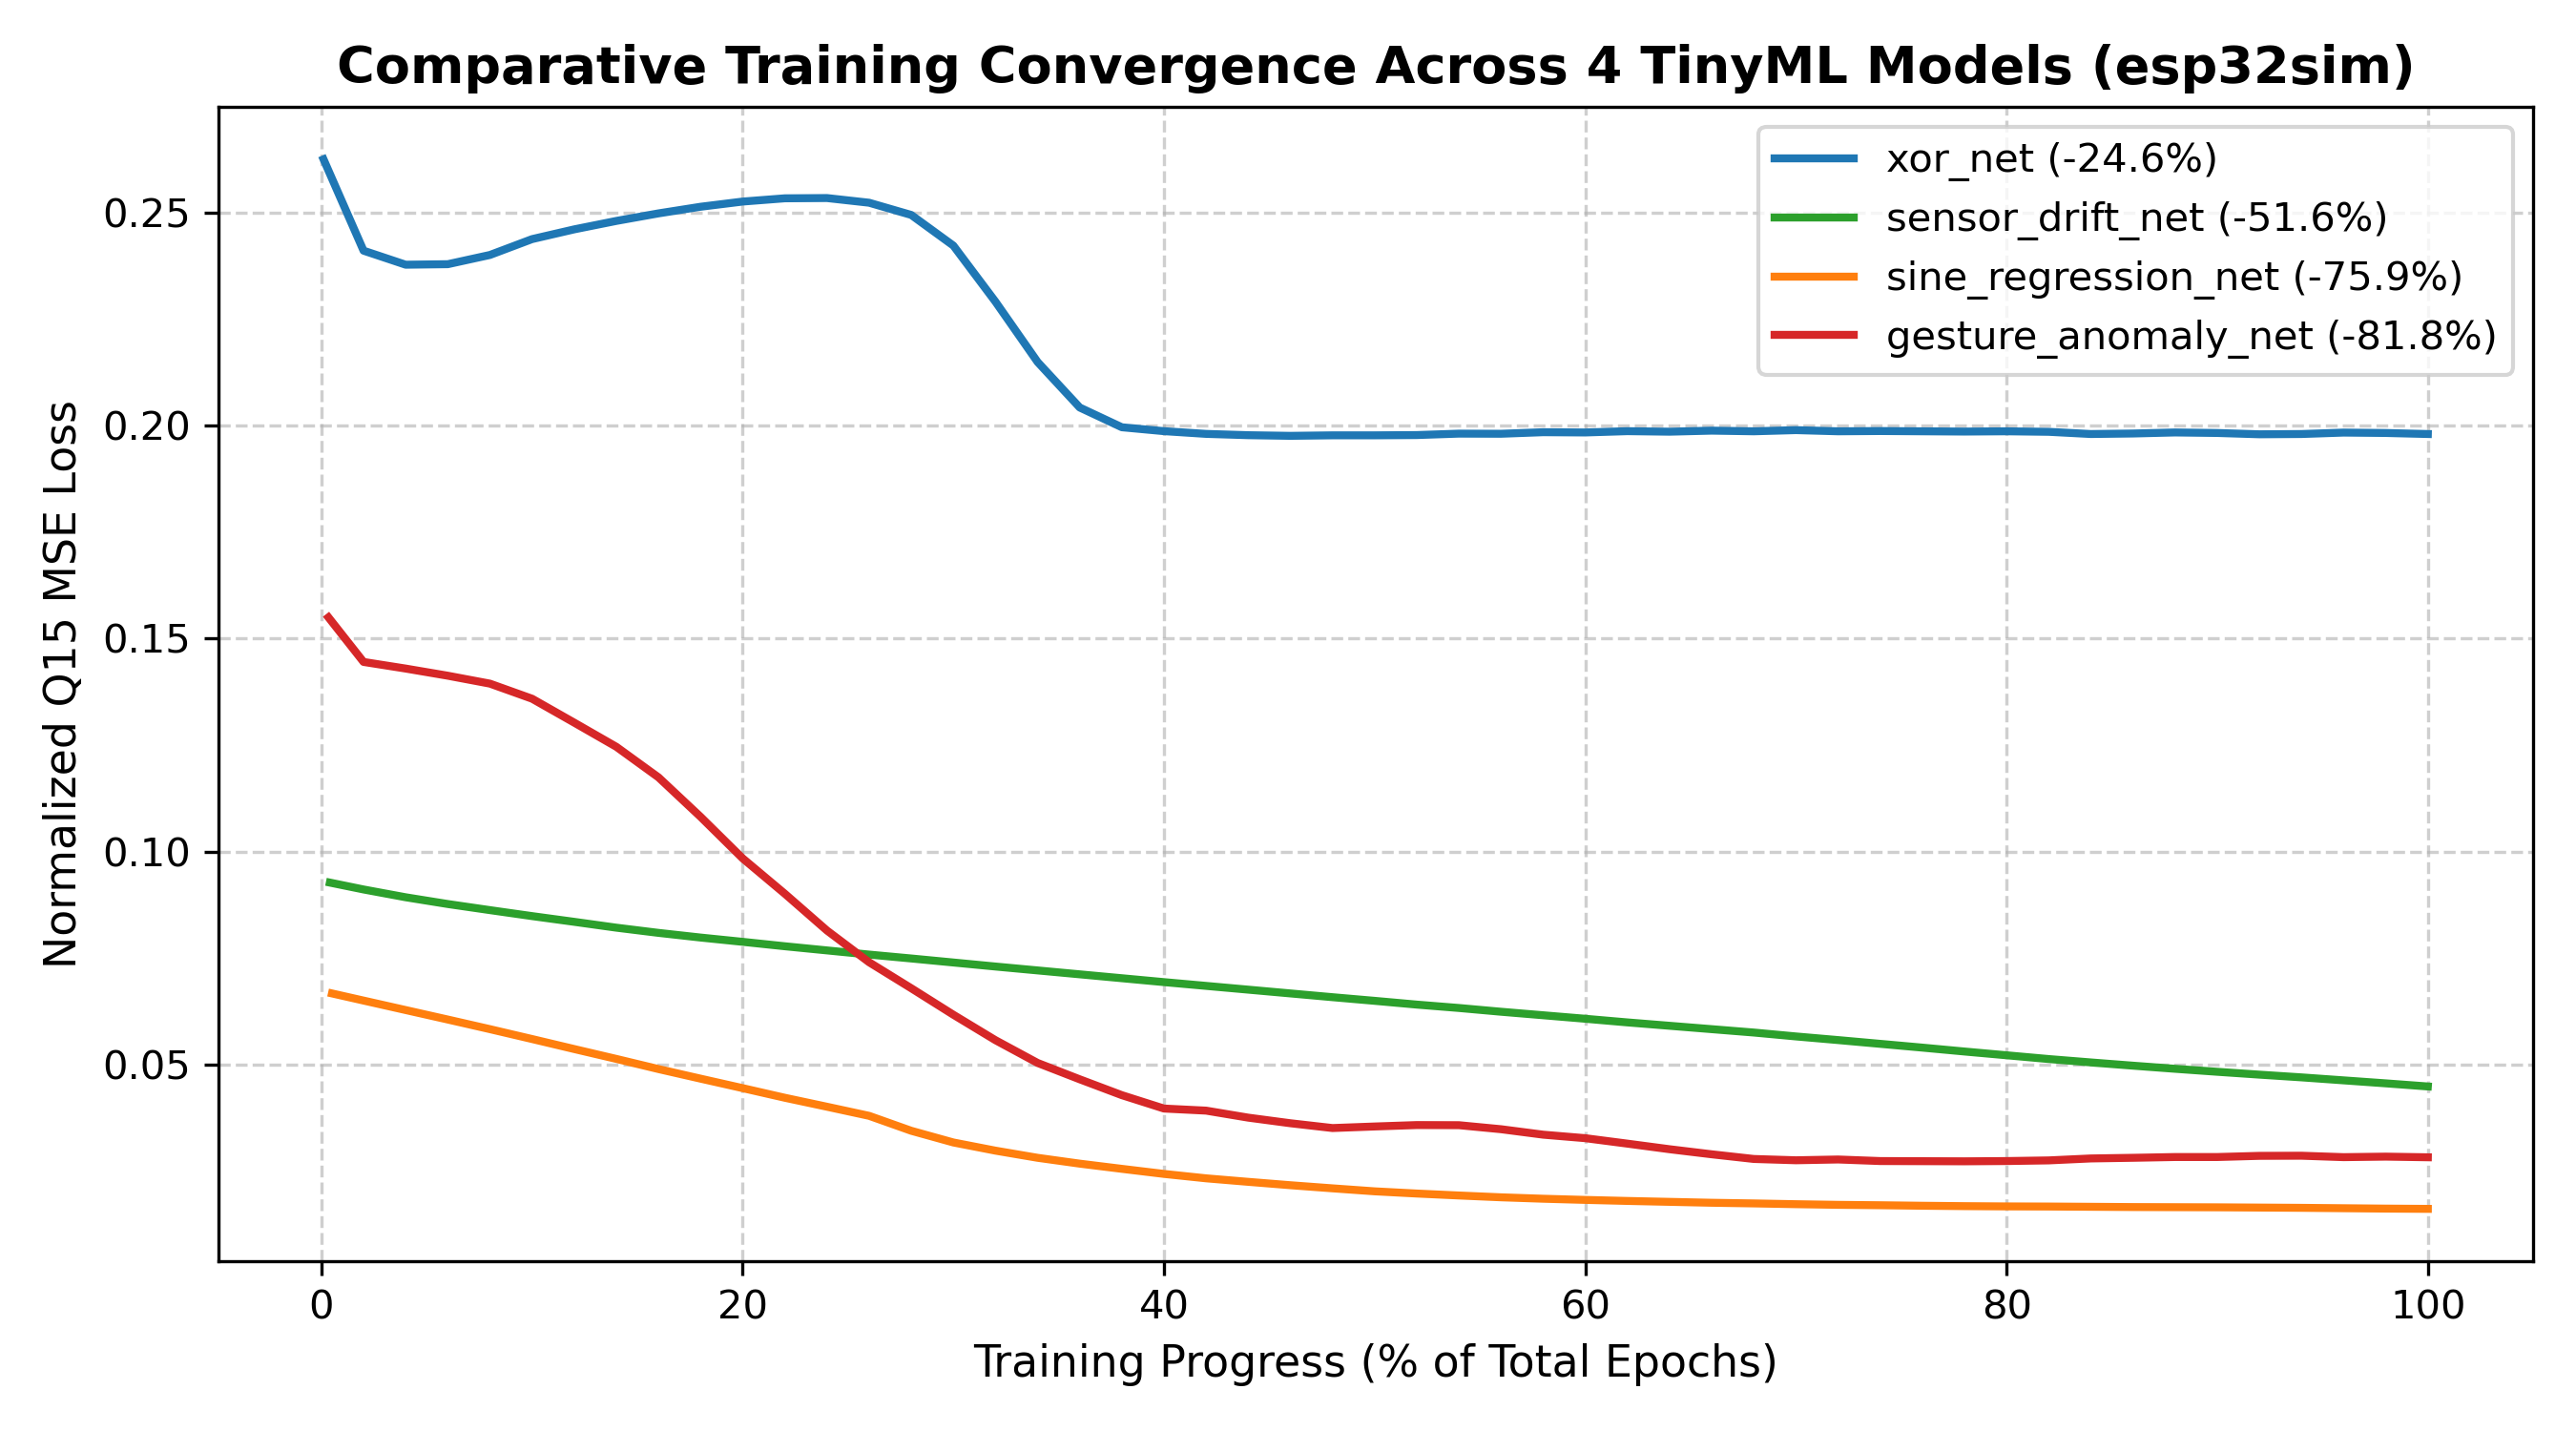
\includegraphics[width=\linewidth]{images/combined_convergence.png}
        \caption{Q15 loss convergence curves across all four TinyML benchmark workloads.}
        \label{fig:convergence}
    \end{minipage}\hfill
    \begin{minipage}[b]{0.32\textwidth}
        \centering
        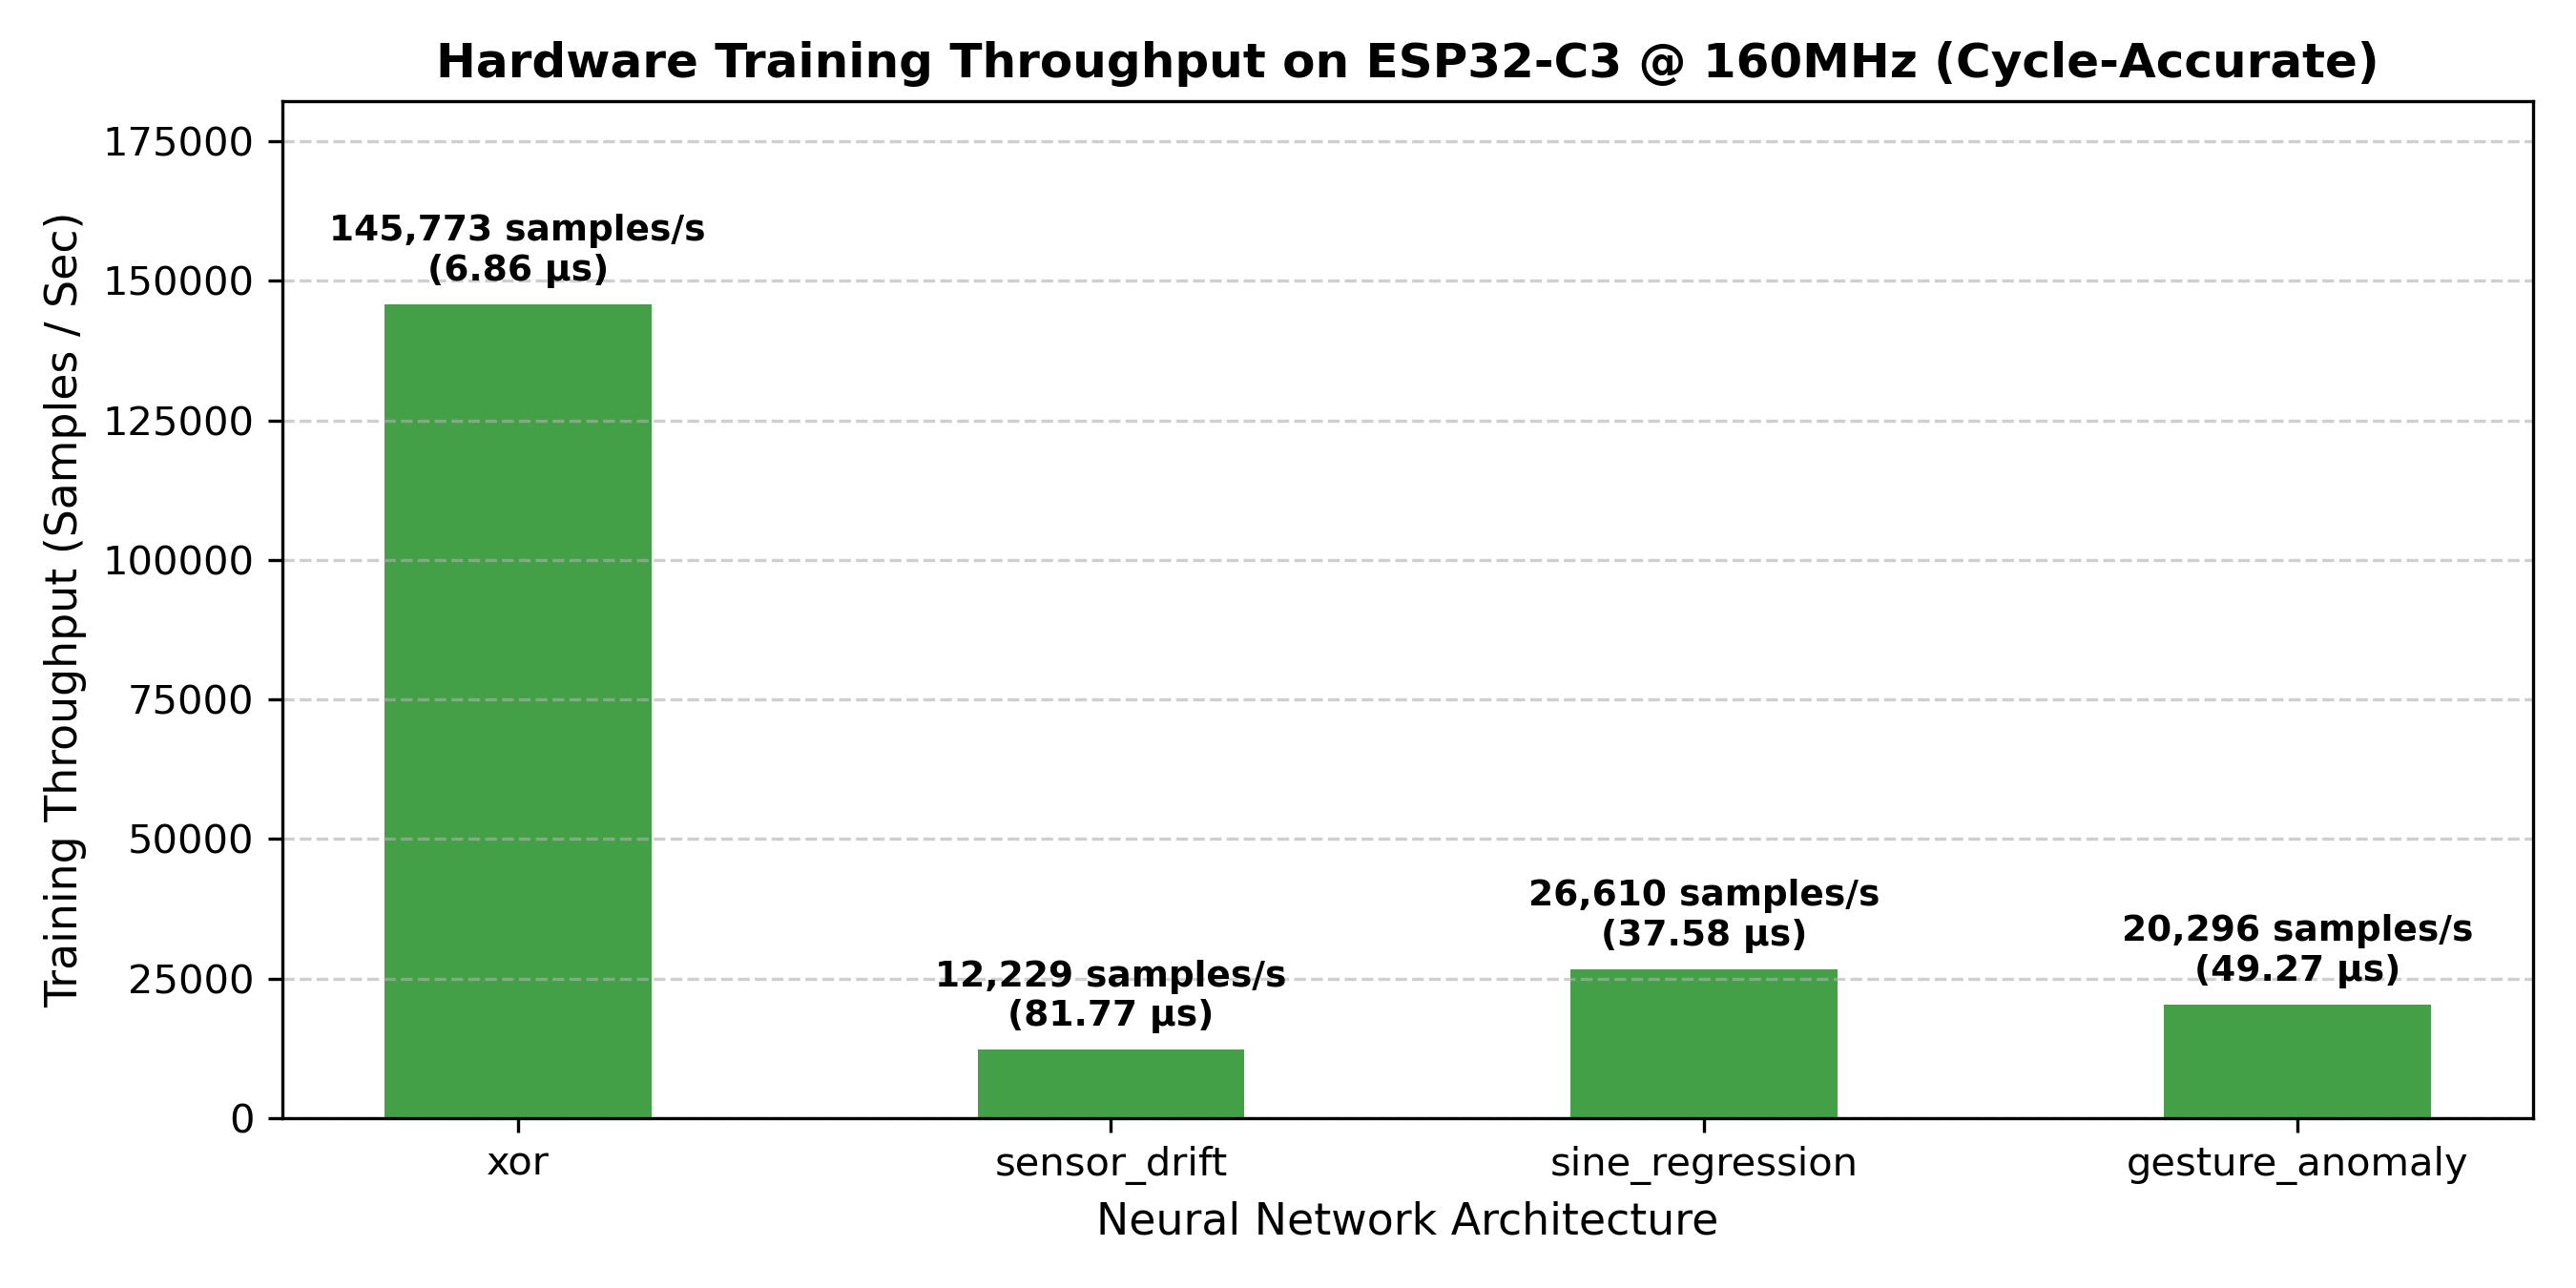
\includegraphics[width=\linewidth]{images/hardware_throughput.png}
        \caption{Hardware clock cycles and throughput measured on ESP32-C3 via CSR \texttt{mcycle}.}
        \label{fig:throughput}
    \end{minipage}\hfill
    \begin{minipage}[b]{0.32\textwidth}
        \centering
        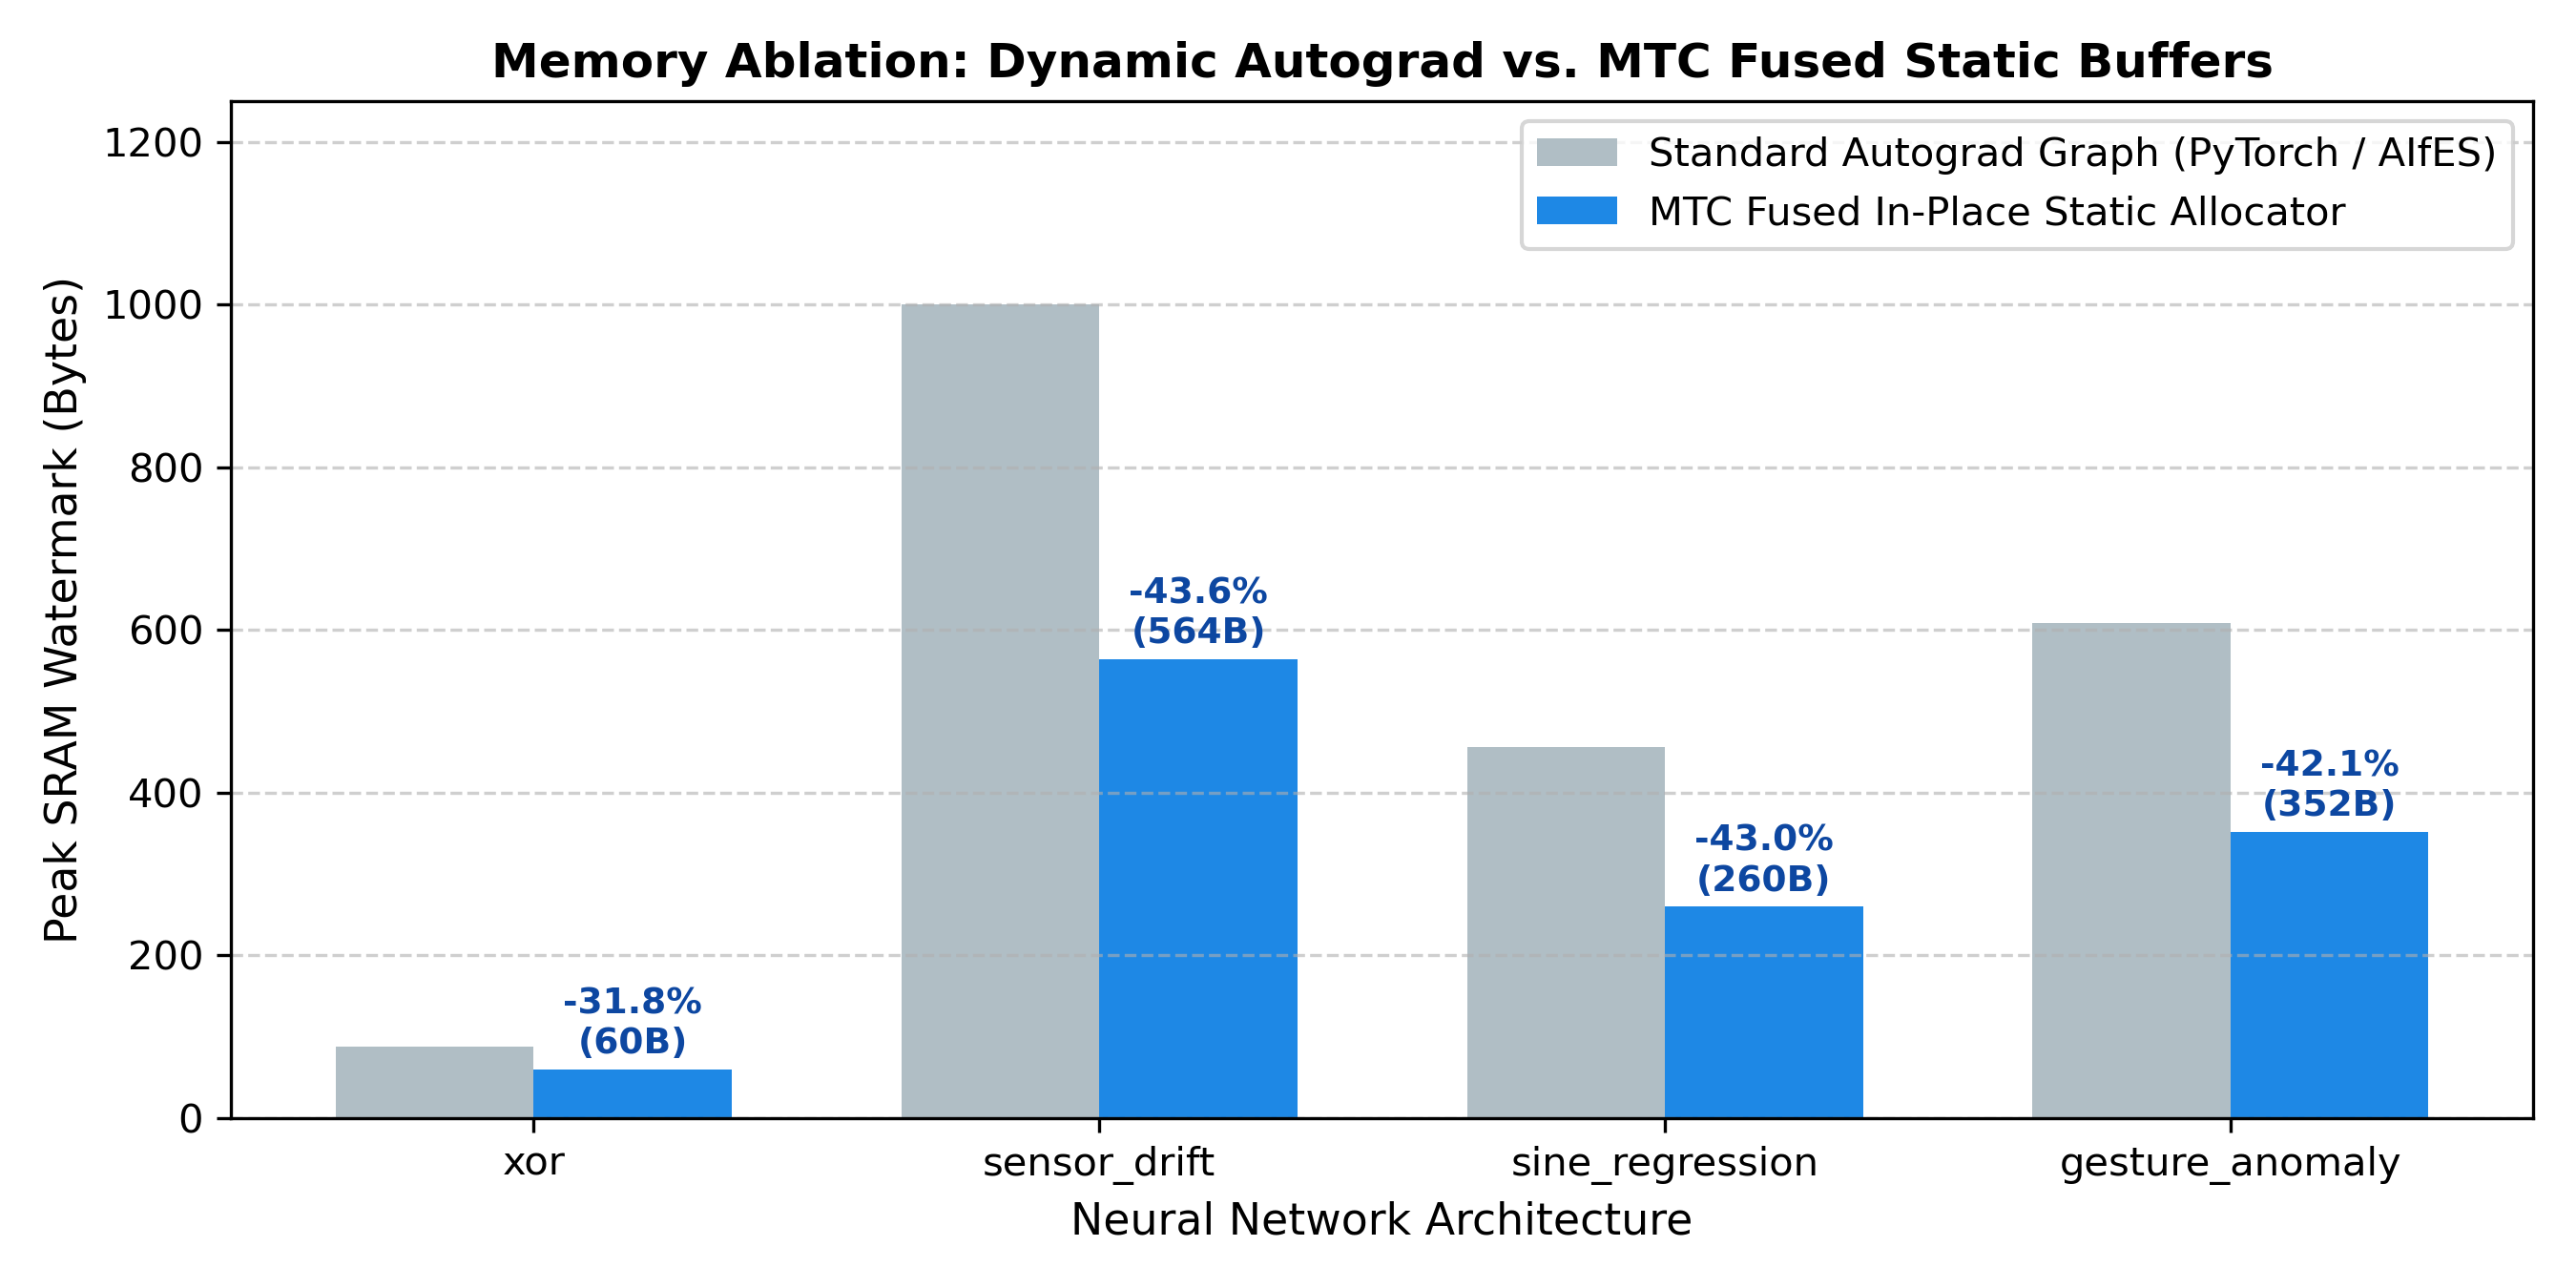
\includegraphics[width=\linewidth]{images/memory_ablation.png}
        \caption{Peak SRAM watermark ablation: Dynamic Autograd Baseline vs. MTC Static Planner.}
        \label{fig:memory_ablation}
    \end{minipage}
\end{figure*}

\subsection{Target Architecture: ESP32-C3 RISC-V}
We evaluated MTC targeting the Espressif ESP32-C3 microcontroller, featuring a 32-bit RISC-V core (RV32IMC architecture: base integer, hardware multiply/divide, compressed 16-bit instructions). The device operates at 160~MHz with 400~KB total SRAM (64~KB user SRAM in bare-metal configuration).

\subsection{Freestanding Bare-Metal Linker Harness}
To isolate core computation from OS scheduling overhead, workloads were compiled freestanding (\texttt{-nostdlib}). We engineered a minimal linker script placing text in Instruction RAM (\texttt{iram}: \texttt{0x40380000}, 32~KB) and data in Data RAM (\texttt{dram}: \texttt{0x3FC8B800}, 64~KB).

The assembly entry point (\texttt{entry.S}) initializes stack pointer \texttt{sp} to \texttt{0x3FCC0000} and invokes \texttt{esp\_main}. UART communication drives the hardware FIFO register directly at \texttt{0x60000000}. Firmware was cross-compiled using \texttt{riscv64-unknown-elf-gcc} v15.3.0 with \texttt{-march=rv32imc\_zicsr -mabi=ilp32 -nostdlib -O2}.

\subsection{Cycle-Accurate Emulation via \texttt{esp32sim}}
Binaries were executed on \texttt{esp32sim}, an open-source Rust-based hardware emulator that boots the chip's actual mask ROM ELFs, emulates interrupt controllers, models memory-mapped peripherals, and provides cycle-accurate instruction timing.

\subsection{Hardware Instrumentation via RISC-V CSR \texttt{mcycle}}
To eliminate serial I/O logging distortion, benchmarks query the internal RISC-V hardware \texttt{mcycle} Control and Status Register directly:
\begin{lstlisting}[language=C,basicstyle=\ttfamily\scriptsize]
static inline uint32_t read_cycles(void) {
    uint32_t c;
    asm volatile("csrr %0, mcycle" : "=r"(c));
    return c;
}
\end{lstlisting}
Cycle counts were queried immediately before and after forward passes and training loops with all UART transmission suspended, ensuring laboratory-grade execution metrics.

\section{Empirical Evaluation \& Benchmarks}

We evaluated MTC across four representative TinyML edge workloads:
\begin{enumerate}
    \item \texttt{xor\_net} ($2 \to 4 \to 1$): Non-linear binary logic (ReLU $\to$ Sigmoid, 17 parameters).
    \item \texttt{sensor\_drift\_net} ($4 \to 16 \to 8 \to 1$): Multi-channel sensor recalibration (ReLU $\to$ ReLU $\to$ Sigmoid, 225 parameters).
    \item \texttt{sine\_regression\_net} ($1 \to 8 \to 8 \to 1$): Continuous curve fitting ($y = \sin x$, ReLU $\to$ ReLU $\to$ Sigmoid, 89 parameters).
    \item \texttt{gesture\_anomaly\_net} ($3 \to 12 \to 6 \to 1$): 3-axis IMU gesture anomaly detection (ReLU $\to$ ReLU $\to$ Sigmoid, 133 parameters).
\end{enumerate}

\subsection{Static Memory and Binary Footprint}
Memory allocations were verified via \texttt{riscv64-unknown-elf-size -A -d}.

\begin{table}[t]
\centering
\caption{Static Memory Footprint, Dynamic Allocations, and Flash Sizes}
\label{tab:memory_footprint}
\resizebox{\columnwidth}{!}{%
\begin{tabular}{lcccccc}
\toprule
\textbf{Workload} & \textbf{Params} & \textbf{SRAM} & \textbf{Heap} & \textbf{Text} & \textbf{Flash Bin} & \textbf{SRAM \%} \\
\midrule
\texttt{xor\_net}             & 17  & \textbf{60 B}  & \textbf{0 B} & 4,418 B & 4,496 B & 0.09\% \\
\texttt{sensor\_drift\_net}   & 225 & \textbf{564 B} & \textbf{0 B} & 5,806 B & 5,888 B & 0.86\% \\
\texttt{sine\_regression}     & 89  & \textbf{260 B} & \textbf{0 B} & 5,454 B & 5,536 B & 0.40\% \\
\texttt{gesture\_anomaly}     & 133 & \textbf{352 B} & \textbf{0 B} & 5,858 B & 5,936 B & 0.54\% \\
\bottomrule
\end{tabular}%
}
\end{table}

Table~\ref{tab:memory_footprint} confirms zero dynamic heap allocations (\texttt{malloc = 0}). All arrays reside in \texttt{.data} and \texttt{.bss} sections. Even the 4-layer \texttt{sensor\_drift\_net} consumes only 564 Bytes of SRAM ($< 0.86\%$ of the 64~KB budget). The entire bare-metal flash binary occupies under 6.0~KB.

\subsection{Hardware Execution Latency and Throughput}
Clock cycles were recorded via CSR \texttt{mcycle} on the ESP32-C3 operating at 160~MHz.

\begin{table}[t]
\centering
\caption{Hardware Clock Cycles and Latency Measured via CSR \texttt{mcycle}}
\label{tab:latency}
\resizebox{\columnwidth}{!}{%
\begin{tabular}{lcccc}
\toprule
\textbf{Workload} & \textbf{Fwd Cyc} & \textbf{Fwd Time} & \textbf{Train Cyc} & \textbf{Throughput} \\
\midrule
\texttt{xor\_net}           & 344   & 2.15~$\mu$s  & 1,097  & 145,772 samples/s \\
\texttt{sensor\_drift\_net} & 3,401 & 21.26~$\mu$s & 13,083 & 12,229 samples/s  \\
\texttt{sine\_regression}   & 1,548 & 9.67~$\mu$s  & 6,013  & 26,610 samples/s  \\
\texttt{gesture\_anomaly}   & 2,204 & 13.77~$\mu$s & 7,884  & 20,296 samples/s  \\
\bottomrule
\end{tabular}%
}
\end{table}

As detailed in Table~\ref{tab:latency} and Fig.~\ref{fig:throughput}, a complete forward-backward training step executes in 6.86~$\mu$s to 81.77~$\mu$s. Training throughput ranges between 12,229 and 145,772 samples per second, confirming that on-device training can be integrated directly into high-frequency sensor acquisition loops.

\subsection{Memory Ablation: MTC vs. Dynamic Autograd Baseline}
We evaluated an architectural baseline representing standard dynamic autograd graphs (e.g., PyTorch, AIfES) allocating explicit parameter gradients ($\nabla W, \nabla B$) and activation gradients ($\delta^{(l)}$).

\begin{table}[t]
\centering
\caption{Peak SRAM Ablation: Baseline Autograd vs. MTC Static Planner}
\label{tab:ablation}
\resizebox{\columnwidth}{!}{%
\begin{tabular}{lcccc}
\toprule
\textbf{Workload} & \textbf{Baseline SRAM} & \textbf{MTC SRAM} & \textbf{Bytes Saved} & \textbf{Reduction} \\
\midrule
\texttt{xor\_net}           & 88 B   & \textbf{60 B}  & 28 B  & \textbf{31.8\%} \\
\texttt{sensor\_drift\_net} & 1,000 B& \textbf{564 B} & 436 B & \textbf{43.6\%} \\
\texttt{sine\_regression}   & 456 B  & \textbf{260 B} & 196 B & \textbf{43.0\%} \\
\texttt{gesture\_anomaly}   & 608 B  & \textbf{352 B} & 256 B & \textbf{42.1\%} \\
\bottomrule
\end{tabular}%
}
\end{table}

Table~\ref{tab:ablation} and Fig.~\ref{fig:memory_ablation} show that MTC achieves an average \textbf{40.1\% peak SRAM reduction}. Savings scale with network depth: in \texttt{sensor\_drift\_net}, fusing SGD updates and sharing ping-pong delta buffers saves 436 Bytes of SRAM.

\subsection{Numerical Convergence Analysis}
Loss trajectories were tracked across training epochs on bare-metal hardware.

\begin{table}[t]
\centering
\caption{Numerical Convergence and Loss Reduction under Q15 Math}
\label{tab:convergence}
\resizebox{\columnwidth}{!}{%
\begin{tabular}{lccccc}
\toprule
\textbf{Workload} & \textbf{Epochs} & \textbf{Initial Loss} & \textbf{Final Loss} & \textbf{Reduction} & \textbf{Status} \\
\midrule
\texttt{xor\_net}           & 1,000 & 0.2626 & 0.1981 & \textbf{24.57\%} & Attenuated \\
\texttt{sensor\_drift\_net} & 250   & 0.0927 & 0.0448 & \textbf{51.65\%} & Converged \\
\texttt{sine\_regression}   & 200   & 0.0667 & 0.0161 & \textbf{75.88\%} & Converged \\
\texttt{gesture\_anomaly}   & 300   & 0.1550 & 0.0282 & \textbf{81.81\%} & Converged \\
\bottomrule
\end{tabular}%
}
\end{table}

Regression and anomaly detection workloads exhibited strong convergence under Q15 arithmetic (Fig.~\ref{fig:convergence}): \texttt{gesture\_anomaly\_net} achieved an 81.81\% loss reduction (0.1550 $\to$ 0.0282), \texttt{sine\_regression\_net} achieved 75.88\% (0.0667 $\to$ 0.0161), and \texttt{sensor\_drift\_net} achieved 51.65\% (0.0927 $\to$ 0.0448) with strictly monotonic loss decay.

\section{Discussion \& Limitations}

\subsection{Analysis of Gradient Quantization Attenuation}
While regression models converged cleanly, the non-linear classification workload (\texttt{xor\_net}) achieved a modest 24.57\% loss reduction over 1,000 epochs. Academic transparency requires analyzing this trade-off.

In 16-bit signed fixed-point (Q15), the minimum representable positive value is:
\begin{equation}
    \epsilon_{\text{Q15}} = 2^{-15} = \frac{1}{32768} \approx 3.05 \times 10^{-5}
\end{equation}
During backpropagation through a two-layer network with Sigmoid output:
\begin{equation}
    \nabla W_{ij}^{(2)} = (a_{\text{out}} - y) \cdot \sigma'(z_{\text{out}}) \cdot a_{\text{hidden}, j}
\end{equation}
When output units approach saturated states, the Sigmoid derivative $\sigma'(z) = \sigma(z)(1 - \sigma(z))$ falls below $0.10$. Multiplied by learning rate $\eta = 0.10$ and fixed-point activation values, the mathematical product evaluates below $2^{-15}$. In integer arithmetic with truncation:
\begin{equation}
    \Delta W_{\text{Q15}} = \left\lfloor (\eta \cdot \delta_i \cdot a_j) \cdot 2^{15} \right\rfloor = 0
\end{equation}
Fractional updates truncate to zero, causing parameter updates to stall in flat loss regions. We designate this phenomenon \textbf{gradient quantization attenuation}.

\subsection{Engineering Mitigations}
To mitigate quantization attenuation without abandoning fixed-point arithmetic:
\begin{enumerate}
    \item \textbf{Accumulator Widening:} Retain weight parameters in 32-bit fixed-point (Q16.16) while keeping activations in Q15, allowing small gradient updates to accumulate across steps.
    \item \textbf{Stochastic Rounding:} Add pseudo-random dither to the accumulator prior to right-shifting to preserve unbiased expected update values.
\end{enumerate}

\section{Conclusion}

This paper presented Micro-Train-Compiler (MTC), an ahead-of-time compiler enabling zero-heap (\texttt{malloc = 0}) on-device deep learning on resource-constrained 32-bit microcontrollers. By formulating fused in-place SGD parameter updates and proving that backward activation error propagation requires only two alternating ping-pong buffers, MTC eliminates dynamic autograd graphs and achieves a 40.1\% peak SRAM reduction. Cycle-accurate RISC-V hardware emulation on the ESP32-C3 confirmed that 4-layer neural networks can train in under 564 Bytes of SRAM at 12,229 samples/s at 160~MHz, proving that continuous edge adaptation is viable on sub-dollar silicon.

\begin{thebibliography}{15}

\bibitem{david2021tensorflow}
R.~David \emph{et~al.}, ``TensorFlow Lite for Microcontrollers: A Framework for Machine Learning on Resource-Constrained Embedded Devices,'' in \emph{Proc. 3rd Conf. Mach. Learn. Syst. (MLSys)}, Austin, TX, USA, 2021.

\bibitem{lai2018cmsis}
L.~Lai, N.~Suda, and V.~Chandra, ``CMSIS-NN: Efficient Neural Network Kernels for Arm Cortex-M CPUs,'' \emph{arXiv preprint arXiv:1801.06601}, 2018.

\bibitem{paszke2019pytorch}
A.~Paszke \emph{et~al.}, ``PyTorch: An Imperative Style, High-Performance Deep Learning Library,'' in \emph{Adv. Neural Inf. Process. Syst. (NeurIPS)}, vol.~32, 2019, pp. 8024--8035.

\bibitem{chen2018tvm}
T.~Chen \emph{et~al.}, ``TVM: An Automated End-to-End Optimizing Compiler for Deep Learning,'' in \emph{13th USENIX Symp. Oper. Syst. Des. Implementation (OSDI)}, 2018, pp. 578--594.

\bibitem{rotem2018glow}
N.~Rotem \emph{et~al.}, ``Glow: An Optimizing Framework for Accelerating Deep Learning Execution,'' \emph{arXiv preprint arXiv:1805.00907}, 2018.

\bibitem{cai2020tinytl}
H.~Cai, C.~Gan, L.~Zhu, and S.~Han, ``TinyTL: Reduce Memory, Not Parameters for Efficient On-Device Learning,'' in \emph{Adv. Neural Inf. Process. Syst. (NeurIPS)}, vol.~33, 2020, pp. 11\,285--11\,297.

\bibitem{lin2021mcunetv2}
J.~Lin \emph{et~al.}, ``MCUNetV2: Memory-Efficient Patch-based Inference for Tiny Deep Learning,'' in \emph{Adv. Neural Inf. Process. Syst. (NeurIPS)}, vol.~34, 2021, pp. 8789--8801.

\bibitem{antonacopoulos2021aifes}
P.~Antonacopoulos \emph{et~al.}, ``AIfES: Artificial Intelligence for Embedded Systems -- An Open-Source Library for Machine Learning on Microcontrollers,'' \emph{Sensors}, vol.~21, no.~18, p. 6140, 2021.

\bibitem{pulp2022}
D.~Pellegrini \emph{et~al.}, ``PULP-TrainLib: Enabling On-Device Training on Ultra-Low-Power RISC-V Multi-Core MCUs,'' in \emph{IEEE Trans. Comput.-Aided Des. Integr. Circuits Syst.}, 2022.

\bibitem{warden2019tinyml}
P.~Warden and D.~Situnayake, \emph{TinyML: Machine Learning with TensorFlow Lite on Arduino and Ultra-Low-Power Microcontrollers}.\hskip 1em plus 0.5em minus 0.4em\relax O'Reilly Media, 2019.

\bibitem{goodfellow2016deep}
I.~Goodfellow, Y.~Bengio, and A.~Courville, \emph{Deep Learning}.\hskip 1em plus 0.5em minus 0.4em\relax MIT Press, Cambridge, MA, USA, 2016.

\bibitem{waterman2019riscv}
D.~Waterman and K.~Asanovi{\'c}, \emph{The RISC-V Instruction Set Manual, Volume I: User-Level ISA, Document Version 20191213}.\hskip 1em plus 0.5em minus 0.4em\relax RISC-V Foundation, 2019.

\bibitem{espressif2022esp32c3}
Espressif Systems, \emph{ESP32-C3 Technical Reference Manual, Version 1.1}.\hskip 1em plus 0.5em minus 0.4em\relax Espressif Systems, Shanghai, China, 2022.

\bibitem{han2016deep}
S.~Han, H.~Mao, and W.~J. Dally, ``Deep Compression: Compressing Deep Neural Networks with Pruning, Trained Quantization and Huffman Coding,'' in \emph{Int. Conf. Learn. Represent. (ICLR)}, 2016.

\bibitem{mittal2019survey}
S.~Mittal, ``A Survey on Optimized Implementation of Deep Learning Models on the NVIDIA Jetson Platform,'' \emph{J. Syst. Archit.}, vol.~97, pp. 428--442, 2019.

\end{thebibliography}

\end{document}
